\documentclass[aspectratio=169]{beamer}
\usepackage[T1]{fontenc}
\usepackage[utf8]{inputenc}

% Enables Portuguese Brasil
\usepackage[portuguese]{babel}

% Enables code listing
\usepackage{listings}

\usepackage{tikz}
\usetikzlibrary{positioning}

%Enables the use of greek letter without a math context
\usepackage{ragged2e}

% Enables math chars
\usepackage{amsmath}

% Enables section slides
\AtBeginSection[]{
	\begin{frame}
	\vfill
	\centering
	\begin{beamercolorbox}[sep=8pt,center,shadow=true,rounded=true]{title}
		\usebeamerfont{title}\insertsectionhead\par
	\end{beamercolorbox}
	\vfill
	\end{frame}
}


%Information to be included in the title page:
\title{Monografia apresentada para cumprimento da disciplina de estudos especiais II}
\author{André Furlan - ensismoebius@gmail.com}
\institute{Universidade Estadual Paulista Júlio de Mesquita Filho}
\date{2023}
\logo{
\includegraphics[height=1cm]{unesp.png}}
\usetheme{Madrid}

\begin{document}
	
	\frame{\titlepage}
	\begin{frame}
		\frametitle{Estrutura da apresentação}
		\begin{itemize}
			\item Introdução.
			\item Revisão de conceitos utilizados.
			\item Trabalhos correlatos.
			\item Cronograma.
		\end{itemize}
	\end{frame}
	
	\section{Introdução}
	
	\begin{frame}
		\frametitle{Autenticação Biométrica de Locutores com Distúrbios Vocais}
		\begin{itemize}
			\item A demanda por mecanismos de autenticação biométrica de locutores (ABLs) é evidente, conforme evidenciado na dissertação \cite{furlan2021caracterizacao}.
			\item Estudos importantes, como \cite{beigi2011speaker} e \cite{neustein2012forensic}, além de publicações em revistas de prestígio, como \cite{hansen2015speaker}, \cite{wang2022racp} e \cite{lee2020two}, comprovam essa demanda.
		\end{itemize}
	\end{frame}
	
	\begin{frame}
		\frametitle{Duas Linhas de Pesquisa Relevantes}
		\begin{itemize}
			\item Autenticação Biométrica de Locutores (ABLs):
			\begin{itemize}
				\item Essa linha de pesquisa tem sido amplamente explorada e conta com obras científicas importantes, como \cite{furlan2021caracterizacao}, \cite{beigi2011speaker} e \cite{neustein2012forensic}.
				\item Métodos e técnicas têm sido propostos para aprimorar a autenticação de locutores por meio do processamento de sinais de voz, como as redes neurais profundas exemplificadas por \cite{mittal2021deep} e \cite{miliaresi2021combining}.
			\end{itemize}
			\item Análise de Sinais de Voz para Pré-diagnóstico e Classificação de Distúrbios Vocais:
			\begin{itemize}
				\item Essa linha de pesquisa se concentra em estratégias acústico-computacionais para identificar e classificar alterações laríngeas e outras irregularidades na fonação, como descrito em \cite{chaiani2022voice} e \cite{fujimura2022classification}.
				\item Metodologias avançadas, como redes neurais profundas \cite{goodfellow2016deep}, e a lógica paraconsistente, como descrito em \cite{fonseca2017linear}, têm sido utilizadas nessa área.
			\end{itemize}
		\end{itemize}
	\end{frame}
	
	\begin{frame}
		\frametitle{Desafio: Autenticar Locutores com Distúrbios Vocais}
		\begin{itemize}
			\item O desafio é autenticar locutores afetados por distúrbios vocais que alteram a impressão acústica da fala, como mencionado em \cite{le2005voz, le2005voz2}.
			\item Distúrbios vocais podem ter origem orgânica, funcional ou orgânico-funcional, e afetam a qualidade e características da voz.
			\item O projeto de pesquisa visa investigar e desenvolver algoritmos biométricos para autenticar locutores com fala severamente degradada devido a esses distúrbios, conforme discutido em \cite{gupta2021residual}.
			\item Uma abordagem promissora é combinar as informações da voz com os sinais cerebrais durante a fonação, ou seja, provenientes da fala imaginada \cite{moctezuma2019subjects}.
		\end{itemize}
	\end{frame}
	
	\begin{frame}
		\frametitle{Escassez de Artigos Científicos}
		\begin{itemize}
			\item Ao pesquisar o tema nos registros do Web of Science e outras bases de dados, observa-se uma escassez de artigos científicos sobre autenticação de locutores com distúrbios vocais.
			\item A maioria dos artigos encontrados são propostas genéricas que envolvem metodologias para viabilizar interfaces cérebro-computador (BCIs), conforme descrito em \cite{rusnac2021eeg} e \cite{brigham2010imagined}.
			\item Por outro lado, os artigos mais relevantes e dedicados à biometria são encontrados nas referências \cite{moctezuma2019subjects, moctezuma2018eeg, jayarathne2016brainid, jayarathne2017survey, del2014electroencephalogram, ruiz2016cerebre}.
		\end{itemize}
	\end{frame}
	
	\section{Objetivos e metas}
	\begin{frame}
		\frametitle{Objetivo Geral}
		O objetivo geral deste trabalho é projetar e implementar algoritmos biométricos capazes de autenticar, por meio da fala, indivíduos que produzem apenas locuções potencialmente degradadas, adicionando informações dos sinais cerebrais durante a fonação (imagined speech).
	\end{frame}
	
	\begin{frame}
		\frametitle{Objetivos Específicos}
		\begin{enumerate}
			\item Realizar um levantamento bibliográfico sobre ABLs com disfonias laríngeas severas (DLSs) e estratégias BCI para imagined speech \cite{10.1117/12.2255697}.
			\item Estudar bases de dados públicas de imagined speech para experimentos iniciais.
			\item Criar uma base de dados contendo sinais de voz de indivíduos com DLS e os respectivos sinais de imagined speech.
		\end{enumerate}
	\end{frame}
	
	\begin{frame}
		\frametitle{Objetivos Específicos (continuação)}
		\begin{enumerate}
			\setcounter{enumi}{3}
			\item Extrair características representativas dos sinais de voz e imagined speech de cada locutor utilizando técnicas de handcrafted extraction e feature learning.
			\item Autenticar os locutores na base de dados usando estruturas de aprendizagem profunda como Redes Neurais Residuais (RNNs) e Deep Spiking Neural Networks (DSNNs).
			\item Implementar os algoritmos em C/C++ para funcionamento off-line e, se possível, em tempo real.
			\item Disseminar os resultados por meio de apresentações em congressos e publicações em periódicos de alto impacto.
		\end{enumerate}
	\end{frame}
		


	\section{Revisão de conceitos utilizados}

	\begin{frame}
		\frametitle{Engenharia paraconsistente de características}
		\only<1>{
			\framesubtitle{Os vetores de características proporcionam uma boa separação interclasses?}
			\begin{columns}
			\column{0.7\textwidth}				
			\begin{figure}
				\centering
				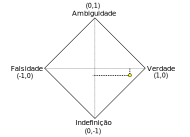
\includegraphics[width=0.6\linewidth,angle=-90]{../monografia/images/paraconsistentPlane}
				\label{fig:paraconsistentplane}
				\caption{Plano paraconsistente}
			\end{figure}
			\column{0.3\textwidth}
			\begin{itemize}
				\item Verdade:\\
				 $\alpha = 1$ e $\beta = 0$.
				\item Ambiguidade:\\
				 $\alpha = 1$ e $\beta = 1$.
				\item Falsidade:\\
				 $\alpha = 0$ e $\beta = 1$.
				\item Indefinição:\\
				 $\alpha = 0$ e $\beta = 0$.
			\end{itemize}
		\end{columns}
		}
		\only<2>{
			\framesubtitle{Cálculo de $\alpha$}
			\begin{figure}
				\centering
				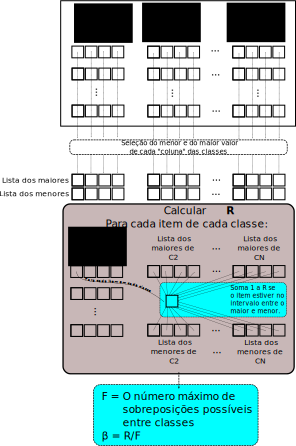
\includegraphics[height=0.8\textheight]{../monografia/images/calculoAlpha}
				\label{fig:calculoalpha}
			\end{figure}
		}
		\only<3>{
			\framesubtitle{Cálculo de $\beta$}
				\begin{figure}
				\centering
				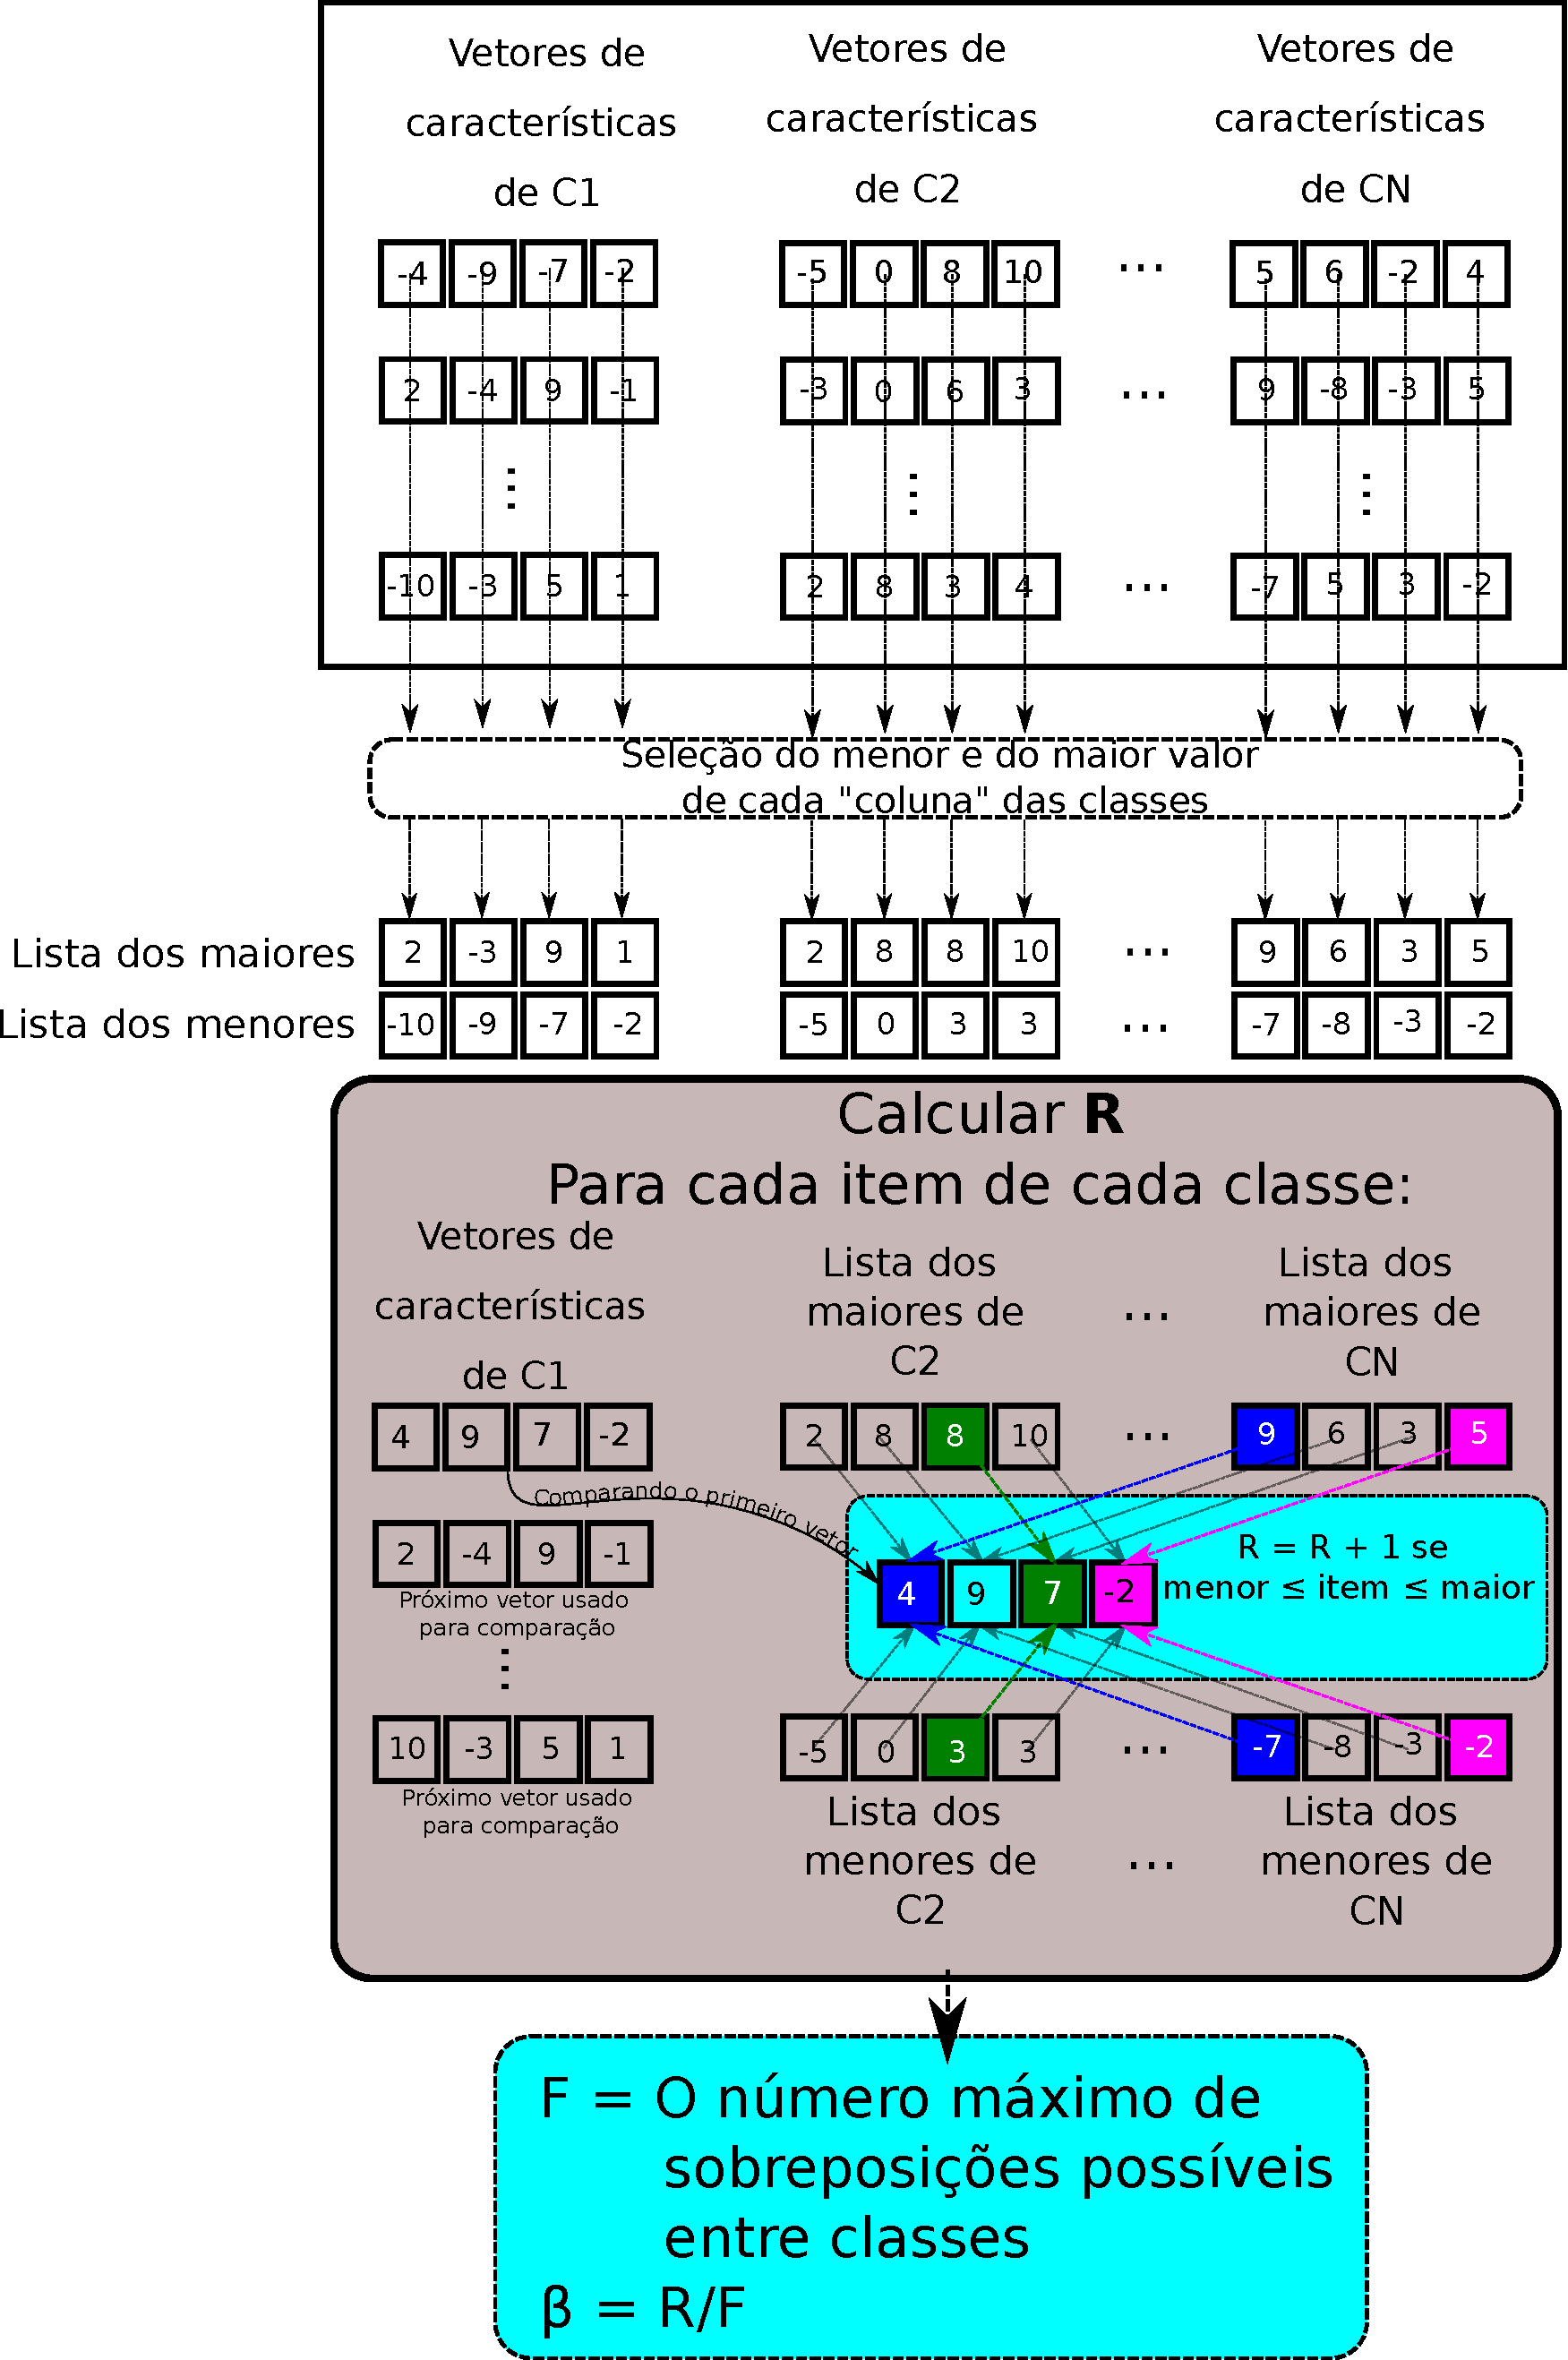
\includegraphics[height=0.8\textheight]{../monografia/images/betaCalculation.pdf}
				\label{fig:calculobeta}
			\end{figure}
		}
		\only<4>{
			\framesubtitle{Graus de certeza e contradição}
			\begin{itemize}
				\item Grau de certeza $\rightarrow G_1=\alpha-\beta $.
				\item Grau de contradição $\rightarrow G_2=\alpha+\beta-1 $.				
			\end{itemize}
			Onde: $-1 \leqslant G_1 \leqslant 1$ e  $-1 \leqslant G_2 \leqslant 1\qquad$.\\
			Seja $P=(G_1,G_2)$
			\begin{itemize}
				\item (-1,0) $\rightarrow$ Falsidade;
				\item (1,0) $\rightarrow$ Verdade;
				\item (0,-1) $\rightarrow$ Indefinição;
				\item (0,1) $\rightarrow$ Ambiguidade.
			\end{itemize}
		}
		\only<5>{
			\framesubtitle{Distancias no plano paraconsistente}
			As distâncias$(D)$ do ponto $P=(G_1,G_2)$ dos limites supracitados. Tal cálculo pode ser feito da seguinte forma:
			\begin{equation*}
			D_{-1,0}=\sqrt{(G_1+1)^2+(G_2)^2}\qquad,
			\end{equation*}
			\begin{equation*}
			D_{1,0}=\sqrt{(G_1-1)^2+(G_2)^2}\qquad,
			\end{equation*}
			\begin{equation*}
			D_{0,-1}=\sqrt{(G_1)^2+(G_2+1)^2}\qquad,		
			\end{equation*}
			\begin{equation*}
			D_{0,1}=\sqrt{(G_1)^2+(G_2-1)^2}\qquad,
			\end{equation*}
		}
	\end{frame}
	
	\begin{frame}
		\frametitle{Filtros digitais \textit{wavelet}}
		\only<1>{
			\framesubtitle{Propriedades}
			\begin{itemize}
				\item Tamanho de janelas variável.
				\item Análise multiresolução.
				\item Análise detalhada em altas e baixas frequências.
			\end{itemize}
		}
		\only<2>{
			\framesubtitle{Restrição de escopo}
			\begin{itemize}
				\item Apenas transformadas diretas.
				\item Não haverá reconstrução do sinal.
				\item Construção de vetores de características.
				\item Domínio discreto.
			\end{itemize}
		}

		\only<3>{
			\framesubtitle{Algoritmo de Malat}
			\begin{itemize}
				\item \textit{Wavelet} Haar: $h[\cdot] = [\frac{1}{\sqrt{2}}, \frac{1}{\sqrt{2}}]$.
				\item Par ortogonal: $g[\cdot] = [\frac{1}{\sqrt{2}}, \frac{-1}{\sqrt{2}}]$.
				\item sinal: $s[\cdot] = [1,2,3,4]$.
			\end{itemize}
			
			\begin{equation*}
			\begin{pmatrix}
			\frac{1}{\sqrt{2}}, \frac{1}{\sqrt{2}}, 0, 0\\
			\frac{1}{\sqrt{2}}, \frac{-1}{\sqrt{2}}, 0, 0\\
			0, 0, \frac{1}{\sqrt{2}}, \frac{1}{\sqrt{2}}\\
			0, 0, \frac{1}{\sqrt{2}}, \frac{1}{\sqrt{2}}\\
			\end{pmatrix} 
			\cdot
			\begin{pmatrix}
			1\\
			2\\
			3\\
			4\\
			\end{pmatrix} 
			=
			\begin{pmatrix}
			\frac{3}{\sqrt{2}}\\
			\frac{-1}{\sqrt{2}}\\
			\frac{7}{\sqrt{2}}\\
			\frac{-1}{\sqrt{2}}\\
			\end{pmatrix}
			\Rightarrow \Big[
			\frac{3}{\sqrt{2}},
			\frac{7}{\sqrt{2}},
			\frac{-1}{\sqrt{2}},
			\frac{-1}{\sqrt{2}}
			\Big]\qquad.
			\end{equation*}
		}

	\end{frame}

	\begin{frame}
		\frametitle{Caracterização dos processos de produção da voz humana}
		\only<1>{
			\framesubtitle{Áreas de estudo}
			\begin{itemize}
				\item Fisiológica ou fonética articulatória.
				\item Acústica ou fonética acústica.
				\item Perceptual.
			\end{itemize}
			\textbf{Foco apenas na acústica}
		}
		\only<2>{
			\framesubtitle{Vozeada versus não-vozeada}
			\begin{itemize}
				\item Vozeada: Pregas vocais.
				\item Não vozeada: Sem pregas vocais.
			\end{itemize}
		}
		\only<3>{
			\framesubtitle{Frequência fundamental da voz}
			\begin{itemize}
				\item Conhecida como $F_0$.
				\item Componente periódico resultante da vibração das pregas vocais.
			\end{itemize}
		}
		\only<4>{
			\framesubtitle{Formantes}
			\begin{itemize}
				\item $F_1 \rightarrow$ amplificação  sonora  na  cavidade  oral  posterior,  posição  da  língua  no  plano  vertical.
				\item $F_2 \rightarrow$ cavidade  oral  anterior,  posição  da  língua  no  plano  horizontal.
				\item $F_3 \rightarrow$ cavidades  à  frente  e  atrás  do  ápice  da  língua.
				\item $F_4 \rightarrow$ formato da laringe e da  faringe.
			\end{itemize}
		}
	\end{frame}

	\begin{frame}
		\frametitle{Redes Neurais}
		\framesubtitle{Autoencoders}
		\begin{columns}[t]
			\begin{column}{0.5\textwidth}
				\begin{itemize}
					\item Consistem em uma função codificadora $h = f(x)$ e uma função decodificadora $r = g(h)$.
					\item A camada oculta $h$ representa uma representação comprimida dos dados de entrada.
					\item Nem sempre o objetivo é aprender uma representação compactada dos dados e reconstruir os dados de entrada com a maior precisão possível.
				\end{itemize}
			\end{column}
			\begin{column}{0.5\textwidth}
				\begin{itemize}
					\item Os autoencoders são limitados para apenas aproximar a entrada e priorizar certos aspectos dos dados.
					\item Podem ser treinados usando técnicas como gradient descent com minibatch ou estocástico.
				\end{itemize}
				\begin{figure}[h]
					\centering
       				\resizebox{\textwidth}{!}{\begin{tikzpicture}[node distance=1.5cm, every edge/.style={draw=black,->}]
	% Nodes
	\node[draw, circle] (x) {$x$};
	\node[draw, rectangle, above right=0.7cm and 1cm of x] (encoder) {Codificador};
	\node[draw, circle, above right=0.7cm and 1cm of encoder] (h) {$h$};
	\node[draw, rectangle, below right=0.7cm and 1cm of h] (decoder) {Decodificador};
	\node[draw, circle, below right=0.7cm and 1cm of decoder] (r) {$r$};
	
	% Arrows
	\draw (x) edge (encoder);
	\draw (encoder) edge (h);
	\draw (h) edge (decoder);
	\draw (decoder) edge (r);
	
	% Loss
	\node[below of=h, yshift=-0.7cm] (loss) {Perda na reconstrução};
	\draw (x) edge (loss);
	\draw (r) edge (loss);
	
	% Labels
	\node[below of=x, yshift=0.7cm] {Entrada};
	\node[below right=0.2cm and 0.8cm of decoder] {Decoder};
	\node[below of=r, yshift=0.7cm] {Entrada reconstruida};
\end{tikzpicture}}
					\label{fig:autoencoder}
				\end{figure}
			\end{column}
		\end{columns}
	\end{frame}
	
	\begin{frame}
		\frametitle{Redes Neurais}
		\framesubtitle{ResNets}
		\begin{columns}[t]
			\begin{column}{0.5\textwidth}
				\begin{itemize}
					\item As ResNets incluem conexões de salto ou mapeamentos de identidade.
					\item Essas conexões permitem que a saída de uma camada seja adicionada diretamente à entrada da camada subsequente.
					\item Permitem que redes mais profundas possam aprender e evitam o problema de \textit{vanishing gradients}.
				\end{itemize}
			\end{column}
			\begin{column}{0.5\textwidth}
				\begin{itemize}
					\item As conexões de salto criam "highway connections" que contornam as camadas intermediárias.
					\item Melhoram o desempenho e a capacidade de aprendizado das redes.
				\end{itemize}
				\begin{figure}
					\centering
					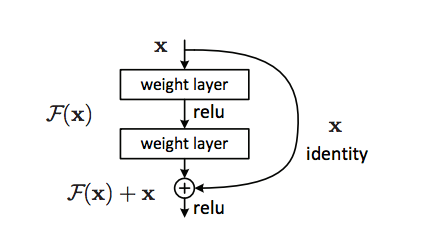
\includegraphics[width=.9\linewidth]{../monografia/images/residualBlock}
					\label{fig:residualblock}
				\end{figure}
			\end{column}
		\end{columns}
	\end{frame}
	
	\begin{frame}
		\frametitle{Redes Neurais}
		\framesubtitle{Spike Neural Networks (SNNs)}
		\begin{itemize}
			\item As SNNs são redes neurais inspiradas na maneira como os neurônios se comunicam no cérebro.
			\item Utilizam picos ou potenciais de ação para representar informações.
			\item As informações são representadas pelo tempo e pela taxa de picos, não pela força das conexões entre os neurônios.
			\item O tempo dos picos e a dinâmica temporal da rede são cruciais no processamento da informação.
			\item Cada pico carrega informações de tempo, permitindo uma codificação mais precisa de informações.
			\item As SNNs são promissoras para a classificação de sinais de voz e EEG devido à natureza temporal desses sinais.
		\end{itemize}
	\end{frame}

	\section{Trabalhos correlatos}
	
	\begin{frame}{Avaliação de um sistema ASR para falantes de língua inglesa com deficiências na fala \cite{WOS:000841879504172}}
		\begin{itemize}
			\item Fonte dos dados ou participantes: 432 falantes da língua inglesa de variadas etnias e deficiências na fala.
			\item Informações ou características extraídas: Energias calculadas a partir de um banco de filtros de 80 dimensões.
			\item Classificadores usados: Rede extratora de características com 8 camadas e rede classificadora LSTM com 2 camadas.
			\item Resultados: Precisão média de reconhecimento de 9\% a 80\%, superando transcritores humanos. Taxa de erro de palavras (WER) média de 4,6\%.
		\end{itemize}
		
	\end{frame}

	
	\begin{frame}{Aumento de dados para reconhecimento de fala disfônica utilizando redes adversariais generativas de convolução profunda (DCGAN) \cite{jin21_interspeech}}
		\begin{itemize}
			\item Fonte dos dados ou participantes: UASpeech.
			\item Informações ou características extraídas: \textit{GAN generator}.
			\item Classificadores usados: \textit{GAN discriminador}.
			\item Resultados: Redução da taxa de erro de palavra (WER) de até 3,05\% em comparação com sistemas sem aumento de dados.
		\end{itemize}
		
	\end{frame}


	\begin{frame}{Detecção de segmentos de palavras imaginadas em sinais de EEG contínuos \cite{WOS:000614122200021}}
		\begin{itemize}
			\item Fonte de dados: Próprias: duas com 27 pessoas e 1 com 20.
			\item Características: Transformada Discreta de Wavelet (DWT), Decomposição Empírica de Modos (EMD), características de energia, dimensões fractais e medidas de caos.
			\item Classificadores: Random Forest (RF), Support Vector Machine (SVM), K-Nearest Neighbors (KNN) e Logistic Regression (LR).
			\item Desempenho: Pontuação média de F1 score de 0,75.
		\end{itemize}
		
	\end{frame}

	\begin{frame}{Combinação de áudio e EEG para aprimorar o reconhecimento de fala em sistemas de Interação Humano-Máquina (HMI) \cite{WOS:000591530700001}}
		\begin{itemize}
			\item Fonte de dados: Kara One \cite{zhao2015classifying}
			\item Características: Múltiplas modalidades (áudio e EEG) e técnicas de Transformada Wavelet (WT).
			\item Resultados: Taxas de precisão de até 74,48\% no reconhecimento de fala.
		\end{itemize}
		
	\end{frame}
		
	\begin{frame}{Uso de técnicas de inteligência artificial (IA) para decodificar a fala a partir de sinais cerebrais humanos \cite{WOS:000857544900001}}
		\begin{itemize}
			\item Modalidade de Dados e Técnicas de IA: Dados de EEG e estímulos de palavras/frases. Técnicas de IA incluem aprendizado de máquina e aprendizado profundo.
			\item Extração de Características e Processamento de Sinais: Técnicas de normalização e extração de características foram aplicadas devido ao ruído nos sinais de EEG. Filtragem de banda passante e técnicas de wavelet foram comumente utilizadas.
			\item Conjunto de Dados e Equipamentos de Gravação: Dispositivos de EEG com 64 canais foram amplamente utilizados, com alguns estudos usando 32 canais ou menos.
		\end{itemize}
		
	\end{frame}
	
	\begin{frame}{Sistema de verificação automática de falas (ASV) para pacientes com disartria \cite{salim2023automatic}}
		\begin{itemize}
			\item Recursos Utilizados: Pitch, volume e probabilidade de vocalização. Aumento de dados fora do domínio.
			\item Conjunto de Dados: Dyarthric Speech Database (DSD) e SpeechDat-Car.
			\item Extração de Características: Vetores de características i-vector e x-vector usando MFCC, variáveis prosódicas e suas combinações.
			\item Resultados: EER de 11,09 para disartria leve, 13,26 na média e 11,97 para disartria grave.
		\end{itemize}
		
	\end{frame}

	\begin{frame}{Uso de redes neurais profundas (DNNs) como criadores de modelos acústicos \cite{6296526}}
		\begin{itemize}
			\item Método: DNNs para geração de vetores de características, posteriormente classificados usando Hidden Markov Models (HMM).
			\item Base de Dados: TIMIT, com mais de 630 falantes da língua inglesa.
			\item Resultados: WER de 18,5\% usando a combinação DNN + HMM.
		\end{itemize}
		
	\end{frame}
	
	\begin{frame}{Uso de modelo de Rede Neural Convolucional (CNN) para classificação de fala \cite{abderrazek20_interspeech}}
		\begin{itemize}
			\item Base de Dados: BREF (fala francesa) e C2SI-LEC (pacientes com falas disfuncionais).
			\item Características Extraídas: Coeficientes Cepstrais de Frequência Mel (MFCCs) e suas derivadas.
			\item Pré-processamento: Normalização dos dados de entrada.
			\item Técnica de Treinamento: Subamostragem aleatória e taxa de aprendizado decaído exponencialmente.
			\item Resultados: Acurácia de 0,68 na base BREF e 0,71 na base C2SI-LEC, superando ouvintes humanos.
		\end{itemize}
		
	\end{frame}

	\begin{frame}{Uso de Rede Neural Recorrente de Memória de Curto Prazo (LSTM-RNN) para decodificação de sinais de EEG \cite{pawar2022wavelet}}
		\begin{itemize}
			\item Dados de EEG: 8 canais de medição dos sinais.
			\item Extração de Características: Transformadas Wavelets nos canais.
			\item Comandos de Áudio: Para cima, para baixo, para a esquerda e para a direita.
			\item Resultados: Acurácia de classificação geral de 92,50\% e métricas adicionais (precisão, \textit{recall} e \textit{F1-score}) com valores próximos.
		\end{itemize}
		
	\end{frame}
	
	\begin{frame}{Uso de EEG e espectroscopia de infravermelho próximo funcional (fNIRS) para coleta de dados \cite{cooney2021bimodal}}
		\begin{itemize}
			\item Extração de Características: Tempo (média, variância, assimetria e curtose) e frequência (densidade espectral de potência e potência de banda).
			\item Classificadores Utilizados: Análise Discriminante Linear (LDA), Máquina de Vetores de Suporte (SVM) e Rede Neural Convolucional (CNN).
			\item Resultados: Precisão de 87,18\% para fala aberta e 53\% para fala imaginada, com destaque para estímulos imagéticos.
		\end{itemize}
		
	\end{frame}
	
	\begin{frame}{Uso de sinais de EEG para fala imaginada e detecção de interações entre regiões do cérebro \cite{bakhshali2022investigating}}
		\begin{itemize}
			\item Dados de EEG: Sinais correspondentes a fala imaginada de quatro vogais.
			\item Extração de Características: Índice de localização (LI) baseado em conectividade funcional entre regiões do cérebro.
			\item Classificadores Utilizados: SVM e Análise Discriminante Linear (LDA).
			\item Resultados: Precisão média da classificação de 81,1\%.
		\end{itemize}
		
	\end{frame}
	
	\begin{frame}{Estrutura baseada em aprendizado métrico profundo para decodificação de \textit{imagined speech} usando interfaces cérebro-máquina (BCI) \cite{lee2021decoding}}
		\begin{itemize}
			\item Bases de Dados: \textit{Coretto} (6 classes) e \textit{BCI Competition} (5 classes).
			\item Extração de Características: Frequência instantânea e entropia espectral dos sinais de EEG.
			\item Estrutura Proposta: Rede Neural Siamesa com aprendizagem métrica profunda.
			\item Resultados: Precisão de 45,00 ± 3,13\% para 6 classes e 48,10 ± 3,68\% para 5 classes.
		\end{itemize}
		
	\end{frame}

	\begin{frame}{Classificação de sinais de EEG correspondentes a falas imaginadas de vogais e palavras \cite{tamm2020classification}}
		\begin{itemize}
			\item Conjunto de Dados EEG: 15 sujeitos imaginando vogais e palavras.
			\item Pré-processamento: Filtragem passa-faixa, subamostragem, segmentação em lotes e normalização.
			\item Classificador Utilizado: Rede Neural Convolucional com transferência de aprendizado.
			\item Resultados: Acurácia de 23,98\% (±3,08).
		\end{itemize}
		
	\end{frame}
	
	\begin{frame}{Uso de \textit{Hashing} sensível a locus (LSH) para reconhecimento de locutor \cite{8396208}}
		\begin{itemize}
			\item Método Proposto: Combinação de MFCC e LSH para identificação do locutor.
			\item Base de Dados: TIMIT 2018.
			\item Procedimentos: Extração de MFCC e criação de tabela \textit{hash} com LSH.
			\item Resultados: Acurácia de 92,66\%.
		\end{itemize}
		
	\end{frame}

	\section{Fechamento}

	\begin{frame}[allowframebreaks]{Fechamento}
		Com base nos estudos mencionados nesta pesquisa, as seguintes abordagens serão consideradas:
		
		\par \textbf{Camada Extratora de Características e Decomposição de Sinais:}
		\begin{itemize}
			\item Utilizar uma camada extratora de características semelhante à abordada por \cite{WOS:000841879504172}.
			\item Aplicar filtros wavelet packet para a decomposição dos sinais.
		\end{itemize}
		
		\par \textbf{Técnicas de Aumento de Dados e Protocolo de Coleta de Dados:}
		\begin{itemize}
			\item Recorrer a técnicas de aumento de dados, como aquelas empregadas por \cite{jin21_interspeech}, devido à escassez de locutores disfônicos.
			\item Adaptar o protocolo de obtenção de dados apresentado por \cite{tamm2020classification}.
			\item Investigar a base de dados UASpeech mencionada por \cite{tamm2020classification}, que pode fornecer informações valiosas para a verificação de padrões.
		\end{itemize}
		
		\framebreak
		
		\par \textbf{Utilização das Transformadas Wavelet e Normalização de Dados:}
		\begin{itemize}
			\item Utilizar diretamente as Transformadas Wavelet para a criação dos vetores de características, seguindo o trabalho de \cite{WOS:000591530700001}.
			\item Considerar técnicas de normalização de dados discutidas por \cite{WOS:000857544900001}.
		\end{itemize}
		
		\framebreak
		
		\par Além disso, os seguintes aspectos interessantes, mas que não necessáriamente serão utilizados, foram observados nos artigos revisados:
		
		\par \textbf{Modelagem Acústica e Conectividade Funcional do Cérebro:}
		\begin{itemize}
			\item O artigo de \cite{6296526} introduz o conceito de Modelagem Acústica, que pode ser relevante para o problema desta pesquisa.
			\item Destaca-se o uso de matrizes que representam a conectividade funcional entre diferentes regiões do cérebro durante a fala imaginada, conforme mencionado por \cite{bakhshali2022investigating}.
		\end{itemize}
		
		\par \textbf{Aprendizado Métrico Profundo:}
		\begin{itemize}
			\item O estudo de \cite{lee2021decoding} propõe uma estrutura baseada em aprendizado métrico profundo para decodificar a fala imaginada, embora essa abordagem difira significativamente da proposta desta pesquisa.
		\end{itemize}
	\end{frame}
	\begin{frame}{Fechamento (Conclusão)}
		\par Em resumo, nenhum dos artigos analisados utiliza, em conjunto, diretamente as técnicas propostas neste estudo, como autoencoders, redes neurais residuais, spike neural networks e vetores de características "hand-crafted". Além disso, nenhum deles tem como objetivo comparar esses métodos, o que torna esta tese potencialmente relevante para a comunidade acadêmica.
	\end{frame}

	\begin{frame}{Cronograma para conclusão do doutorado}
			\par Até a presente data foram realizados os levantamentos bibliográficos e o cumprimento dos créditos necessários em disciplinas para o Doutorado.
			
			\par \textbf{Fases do Projeto:}
			
			\begin{itemize}
				\item \textbf{E1:} Levantamento bibliográfico sobre aquisição e análise de \textit{imagined speech} por meio de EEG e reconhecimento de voz em pacientes com disfonia.
				\item \textbf{E2:} Diálogos com profissionais de fonoaudiologia e neurologia, estudo de base de dados pública e criação de uma base de dados própria.
				\item \textbf{E3:} Pré-processamento e extração de características representativas dos sinais de voz e \textit{imagined speeches}.
				\item \textbf{E4:} Integração das etapas de extração de características e autenticação utilizando estruturas de aprendizado profundo.
				\item \textbf{E5:} Apresentação dos experimentos em eventos científicos, publicação dos resultados e elaboração da monografia de qualificação e tese de doutorado.
			\end{itemize}
	\end{frame}

	\begin{frame}{Cronograma para conclusão do doutorado}
		\begin{columns}[onlytextwidth]
			\begin{column}{0.33\textwidth}
				\centering
				\resizebox{\linewidth}{!}{
					\begin{tabular}{|c|c|c|c|c|c|}
		                \hline
           				{Mês/Ano} & {E1} & {E2} & {E3} & {E4} & {E5} \\
           				\hline
         				09/22 & X & & & & \\
           				10/22 & X & & & & \\
           				11/22 & X & & & & \\
           				12/22 & X & & & & \\
           				01/23 & X & X & & & \\
           				02/23 & X & X & & & \\
           				03/23 & X & X & & & \\
           				04/23 & X & X & & & \\
           				05/23 & X & X & & & X \\
           				06/23 & X & X & & & X \\
           				07/23 & & X & X & & X \\
           				08/23 & & X & X & & X \\
           				09/23 & & X & X & & \\
           				10/23 & & X & X & & \\
           				11/23 & & X & X & & \\
						12/23 & & X & X & & \\
						\hline
					\end{tabular}
				}
			\end{column}
			\begin{column}{0.33\textwidth}
				\centering
				\resizebox{\linewidth}{!}{
					\begin{tabular}{|c|c|c|c|c|c|}
		                \hline
						{Mês/Ano} & {E1} & {E2} & {E3} & {E4} & {E5} \\
						\hline
						01/24 & & X & X & X & X \\
						02/24 & & X & X & X & X \\
						03/24 & & & X & X & \\
						04/24 & & & X & X & \\
						05/24 & & & X & X & \\
						06/24 & & & X & X & \\
						07/24 & & & X & X & \\
						08/24 & & & X & X & \\
						09/24 & & & X & X & \\
						10/24 & & & X & X & \\
						11/24 & & & X & X & \\
						12/24 & & & X & X & \\
						01/25 & & & X & X & \\
						02/25 & & & X & X & \\
						03/25 & & & X & X & \\
						04/25 & & & X & X & \\
						\hline
					\end{tabular}
				}
			\end{column}
			\begin{column}{0.33\textwidth}
				\centering
				\resizebox{\linewidth}{!}{
					\begin{tabular}{|c|c|c|c|c|c|}
						\hline
						{Mês/Ano} & {E1} & {E2} & {E3} & {E4} & {E5} \\
						\hline
						05/25 & & & X & X & \\
						06/25 & & & X & X & \\
						07/25 & & & X & X & \\
						08/25 & & & X & X & \\
						09/25 & & & X & X & \\
						10/25 & & & X & X & \\
						11/25 & & & X & X & \\
						12/25 & & & X & X & \\
						01/26 & & & X & X & \\
						02/26 & & & X & X & \\
						03/26 & & & X & X & \\
						04/26 & & & X & X & \\
						05/26 & & & & & X \\
						06/26 & & & & & X \\
						07/26 & & & & & X \\
						08/26 & & & & & X \\
						\hline
					\end{tabular}
				}
			\end{column}
		\end{columns}
	\end{frame}

	\begin{frame}[allowframebreaks]
		\frametitle{Referências}
		\bibliography{../monografia/bibliography.bib}
		\bibliographystyle{alpha}
	\end{frame}
	
\end{document}